\documentclass{ntmanuscript}
%\usepackage[acronym,toc]{glossaries}
%\include{acros}
%\makeglossaries
%%%%%%%%%%%%%%%%%%%%%%%%%%%%%%%%%%%
\title{Facility Deployment Decisions through Warp Optimizaton
       of Regressed Gaussian Processes}

% Authors. Separated by commas
\author{Anthony Michael Scopatz$^1$}

% Institutes of the authors
\institute{$^1$University of South Carolina, Department of Mechanical 
    Engineering, Nuclear Engineering Program, Columbia, SC 29201}



% Information concerning the person submitting the manuscript
\submitter{Anthony M. Scopatz}
\submitteraddress{541 Main Street, Columbia, SC 29208}
\submitteremail{scopatz@cec.sc.edu}


% No more than three keywords, though each can be a phrase
\keywords{nuclear fuel cycle, gaussian process, dynamic time warping}

\usepackage{color}
\usepackage{graphicx}
\usepackage{booktabs} % nice rules for tables
\usepackage{microtype} % if using PDF
\usepackage{xspace}
\usepackage{listings}
\usepackage{textcomp}
\usepackage{ulem}
\usepackage{hyperref}
\usepackage{amssymb}
\DeclareMathAlphabet{\mathpzc}{OT1}{pzc}{m}{it}

\definecolor{listinggray}{gray}{0.9}
\definecolor{lbcolor}{rgb}{0.9,0.9,0.9}
\lstset{
    %backgroundcolor=\color{lbcolor},
    %language={C++},
    language={Python},
    tabsize=4,
    rulecolor=\color{black},
    upquote=true,
    aboveskip={1.5\baselineskip},
    belowskip={1.5\baselineskip},
    columns=fixed,
    extendedchars=true,
    breaklines=true,
    prebreak=\raisebox{0ex}[0ex][0ex]{\ensuremath{\hookleftarrow}},
    frame=single,
    showtabs=false,
    showspaces=false,
    showstringspaces=false,
    basicstyle=\scriptsize\ttfamily\color{green!40!black},
    keywordstyle=\color[rgb]{0,0,1.0},
    commentstyle=\color[rgb]{0.133,0.545,0.133},
    stringstyle=\color[rgb]{0.627,0.126,0.941},
    numberstyle=\color[rgb]{0,1,0},
    identifierstyle=\color{black},
    captionpos=t,
}

\newcommand{\code}[1]{\lstinline[basicstyle=\ttfamily\color{green!40!black}]|#1|}
\newcommand{\units}[1] {\:\text{#1}}%
\newcommand{\SN}{S$_N$}
\newcommand{\cyclus}{\textsc{Cyclus}\xspace}
\newcommand{\Cyclus}{\cyclus}
\newcommand{\citeme}{\textcolor{red}{CITE}\xspace}
\newcommand{\cycpp}{\code{cycpp}\xspace}
\newcommand{\TODO}[1] {{\color{red}\textbf{TODO: #1}}}%

\newcommand{\comment}[1]{{\color{green}\textbf{#1}}}

\newcommand{\E}{\mathbb{E}}
\newcommand{\GP}{\mathpzc{GP}}
\newcommand{\N}{\mathbb{N}}
\newcommand{\LWR}{\mathrm{LWR}}
\newcommand{\FR}{\mathrm{FR}}
\newcommand{\Total}{\mathrm{Total}}
\newcommand{\argmin}{\mathrm{argmin}}
\newcommand{\CYCLUS}{\mathrm{Cyclus}}
\newcommand{\DYMOND}{\mathrm{DYMOND}}
\newcommand{\I}{\mathbf{I}}
\newcommand{\K}{\mathbf{K}}
\newcommand{\stochastic}{\texttt{`stochastic'}\xspace}
\newcommand{\innerprod}{\texttt{`inner-prod'}\xspace}
\newcommand{\allflag}{\texttt{`all'}\xspace}



\date{}
%%%%%%%%%%%%%%%%%%%%%%%%%%%%%%%%%%%
\begin{document}

\begin{abstract}
A method for quickly determining deployment schedules that meet a given 
fuel cycle demand is presented here. This algorithm is fast enough to 
perform \emph{in situ} in low-fidelity fuel cycle simulators. It uses
Gaussian process regression models to predict the prodcution curve as a 
function of time and the number of deployed facilites. The each of these
predictions is measured against the demand curve using the dynamic time
warping distance. The minium distance deployment schedule is evaluated
in a full fuel cycle simulation, whose generated prodcution curve 
then informs the model on the next optimization iteration. The method
converges with five to ten iterations to a total distance less than one 
percent of the total deployable production. A representative once-through
fuel cycle is used to demonstrtate the methodology.
\end{abstract}

\section{Introduction}
\label{intro}

With the recent advent of agent-based nuclear fuel cycle simulators, such as 
Cyclus \cite{DBLP:journals/corr/HuffGCFMOSSW15,cyclus_v1_0}, there comes the 
possibility to make \emph{in situ} facility deployment decisions. This 
agency would more fully model real-world fuel cycles, where institutions
predict future demand and choose their future deployment schedules 
approriately. However, one of the major challenges to making \emph{in situ}
deployment decisions is the speed at which ``good enough'' decisions can 
be made. This paper proposes three related deployment-specific optimization 
algorithims that can be used for any facility type.

The demands of a fuel cycle scenario can often be simply stated, e.g. 
1\% growth in power production [GWe]. Picking a deployment schedule for a 
certain kind of facility (e.g. reactors) can thus be seen as an optimization 
problem of how well the deployment schedule meets the demand. Here, the 
dynamic time warping (DTW) \cite{muller} distance is minimized 
between the demand curve and the regression of a Gaussian Process model (GP) 
\cite{rasmussen2006gaussian} of prior simulations. This minimization produces
a guess for a deployment schedule which is subsequently tested using 
the actual simulator. This process is repeated until an optimal deployment
schedule for the given demand is found.

Importantly, by using the Gaussian process surrogates, the number of 
simulation realizations that must be executed as part of the optimization is 
reduced to only a handful. Furthermore, it is at least two 
orders-of-magnitude faster to test the model than it is to run a single
low-fidelity fuel cycle simulation. Because of the realtive cheapness, it 
is suitable to be used inside of a fuel cycle simulation. Traditional
\emph{ex situ} optimizers may be able to find more precise solutions but at a
computational cost beyond the scope and need of an \emph{in situ} use case.

Every iteration of warp optimization of regressed Gaussian processes (WORG) 
method described here has two phases. The first is an esitmation phase where 
the Gaussian process model is built and evaluated. The second takes the 
deployment schedule from the estimation phase and run it in a fuel cycle 
simulator. The results of the simulator of the $s$-th iteration are then 
used to inform the model on the $(s+1)$-th iteration. 

Inside of each estimation phase there are three possible strategies for 
chosing the next deployment schedule.  The first is to sample of the 
space of all possible deployment strategies stochatically and then take the 
best guess.  The second is to search through the inner product of all choices,
picking the best option for each deployment parameter. The third option 
is to perform the previous two strategies and determine which one picked
has the better guess.


Challenges with this formulation
inetger capacities, discrete deployments, no jacobian, combinatorical
\section{The WORG Method}
\label{method}

In order to describe the WORG method, first it is is useful to define  
notation for demand curves and their parameterization.  Call $t$ the time
[years] up to some maximal time $T$ (e.g. 50 years) over which the time 
demand curve is know.  Then call $f(t)$ the demand curve, in the natural 
units of the facility type ([GWe] for reactors).
$f(t)$ may be any function that is desired, including non-differential 
functions. For example, though, the demand curve for a 1\% growth rate 
starting at 90 [GWe] has the following form:
\begin{equation}
\label{f-1}
f(t) = 90\times 1.01^t
\end{equation}
Additionally, call $\Theta$ the deployment schedule for the facility.
$\Theta$ is a sequence of $P$ parameters, indexed by $p$, as seen in 
Equation \ref{Theta}.
\begin{equation}
\label{Theta}
\Theta = \left\{\theta_1, \theta_2, \ldots, \theta_P\right\}
\end{equation}
Each $\theta_p$ represents that number of facilities to deploy on its
time step. In simple cases where there is only one type of facility
to deploy $P == T$.  However, when the deployment schedules of multiple 
facility types are needed to meet the same demand curve, $P > T$.  The usual
example is for transition scenarios which necessarily require multiple kinds
of reactors.

Now denote $M$ as the sequence for the minimum number of facilities deployable
for the $p$-th deployment. Then call $N$ the sequence of the maximum number
of facilcities deployable. The deployment parameters are thus each defined
on the range $\theta_p \in [M_p, N_p]$. Furthermore, because only whole
numbers of facilities may be deployed $\theta_p \in \N$.  It is also typical, 
but not required for $M = \mathbf{\vec{0}}$, which is also the lower bound
for all possible $\theta_p$ since faciliteis may not be retired by the 
deployment schedule.

From here, call $g(t, \Theta)$ the production as a function of time for a
given deployment facility. This has the same units as the demand curve.
Thus for power demand and reactor deployments $g$ is in [GWe]. The 
optimization problem can now be posed as an attempt to find a $\Theta$
that minimizes the difference between $f$ and $g$.

\subsection{Dynamic Time Warping}
\label{dtw}

The question of how to take the difference between the demand curve and 
the production curve is an important one. The na\"ive option is to simply 
take the $L_1$ norm of the difference between these two time sereies, as 
seen in Equation \ref{delta-l1}.  However, since $g(t, \Theta)$ for 
a simulation is expensive compute, any operation that can meaningfully 
exacerbate the difference betweeen time series helps drive down the number 
of optimization iterations.

Dynamic time warping is just such a mechanism. It computes 
a distance between any two time series which compounds the separartion 
between the two. Additionally, the time series are not required to be of the 
same length, though for optimization purposes there is no reason for them 
not to be. DTW gives a measure of amount that one time series would need to 
be warped to become the other time series. It is, therefore, a holistic  
measure that operates over the complete time series. Dynamic time warping
is more fully covered in \cite{muller}.  However, an 
optimization-relevant introduction is given here.

For the time series $f$ and $g$, there are three parts to dynamic time 
warping. The first is the distance $d$, which will be minimized. The second 
is a cost matrix $C$ that helps compute $d$ by indicating how far a point 
on $f$ is from another point on $g$. Thirdly, the warp path $u$ is the 
minimal cost curve through the $C$ matrix from the fist point in time to 
the last. The DTW distance can thus be interpreted as the 
total cost of travelling the warp path.

The first step in computing a dynamic time warp distance is to 
assemble the cost matrix. Say that the demand time series $f$ has 
length $A$ indexed by $a$ and the production time series $g$ has 
length $B$ indexed by $b$. For the optimization problem here, $A$ and $B$
are in practice both equal to $T$.  However, it is useful to have $a$ and 
$b$ index the two time series separately. Now denote an $A\times B$ matrix 
$\Delta L$ as the $L_1$ norm of the difference between $f$ and $g$:
\begin{equation}
\label{delta-l1}
\Delta L_{a,b} = \left|f(a) - g(b, \Theta)\right|_1
\end{equation}
The cost matrix $C$ may now be defined as the $A\times B$ sized matrix 
which follows the recursion relations seen in Equation \ref{cost-matrix}.
\begin{equation}
\label{cost-matrix}
\begin{split}
C_{1,1} & = \Delta L_{1,1}\\
C_{1,b+1} & = \Delta L_{1,b} + C_{1,b}\\
C_{a+1,1} & = \Delta L_{a,1} + C_{a,1}\\
C_{a+1,b+1} & = \Delta L_{a,b} + \min\left[C_{a,b}, C_{a+1,b}, C_{a,b+1}\right]
\end{split}
\end{equation}
The boundary conditions above are the same as setting an infinite cost to 
any $a \le 0$ or $b \le 0$. The cost matrix $C$ has the same units as the 
demand curve. However, the scale of $C$ is (except for the fiducial case) 
larger than the demand. This is because the cost matrix compounds the 
minimum value of previous entries. 

Knowing a cost matrix, the warp path can be computed by traversing the 
matrix backwards from the $(A, B)$ corner to the $(1, 1)$ corner.
If the length of the warp is $I$ indexed by $i$, the warp path itself 
can be thought of as a sequence of coordinate points $u_i$. For a given 
point $u_i$ in the warp path, the previous point $u_{i-1}$ found by 
picking the minimum cost point among the locations one column over $(a,b-1)$, 
one row over $(a-1,b)$, and one previous diagonal element to $(a-1,b-1)$. 
Equation \ref{warp-path} expresses this mathematically.
\begin{equation}
\label{warp-path}
u_{i-1} = \argmin\left[C_{a-1,b-1}, C_{a-1,b}, C_{a,b-1}\right]
\end{equation}
The maximum possible length of $u$ is thus $\max(I) = A + B$.
The minimum possible length, though, is $\min(I) = \sqrt{A^2 + B^2}$. 

The dynamic time warping distance distance $d$ can now be stated as the 
cost of the final entry of the warp path normalized by the maximum possible
length of the warp path.  
\begin{equation}
\label{d-calc-ab}
d(f, g) = \frac{C_{A,B}}{A + B}
\end{equation}
However, because the demand curve and the production curve that is predicted
or calculated are typically defined on the same time grid, $d$ can be further
reduced to the following:
\begin{equation}
\label{d-calc}
d(f, g) = \frac{C_{T,T}}{2T}
\end{equation}
Therefore, $d$ has the same units as the demand curve, production curve, 
and cost matrix.

As an example, take 1\% growth that starts with 90 GWe in the year 
2016 as the demand curve. Then consider a production curve that 
under produces the demand by 5\% for 25 years before switching to over 
producing this curve by 5\% for the next 25 years.  
Figure \ref{cost-demand-to-production} shows the dynamic time warping 
between these two.

\begin{figure}[htb]
\centering
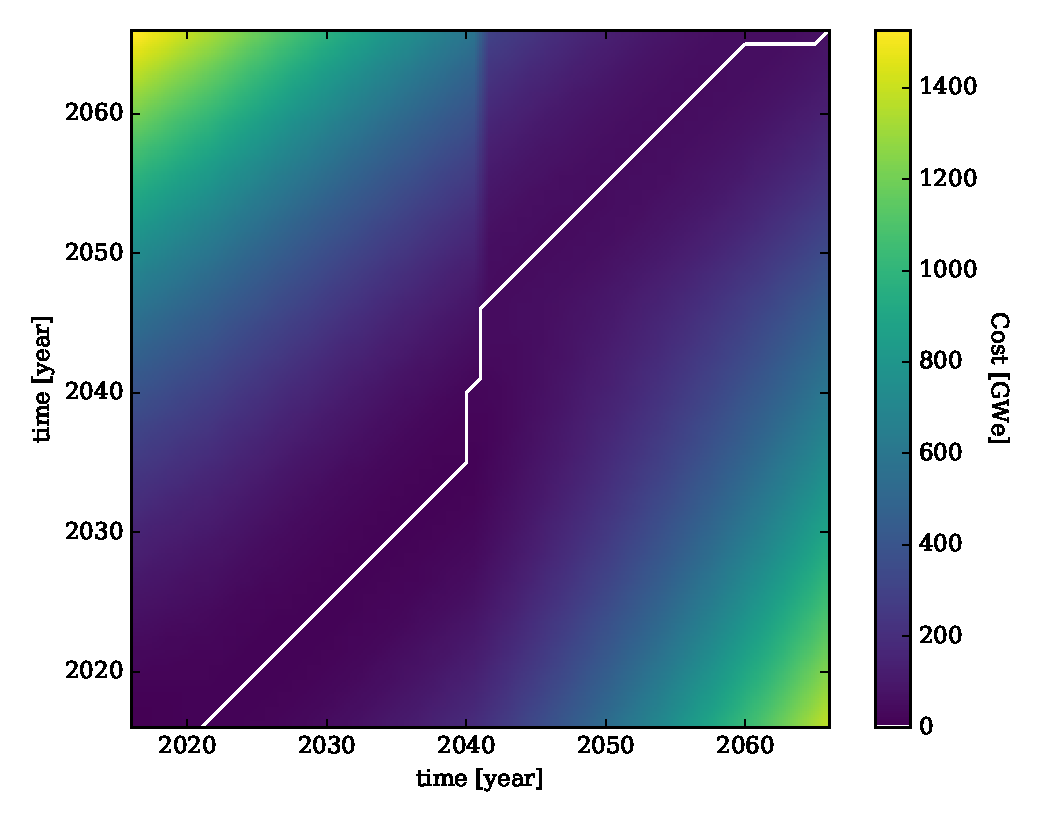
\includegraphics[width=0.9\textwidth]{cost-demand-to-production.eps}
\caption{Heat map of the cost matrix between a 1\% growth demand curve and 
a production curve the under produces by 5\% for the first 25 years and then
over produces for the second 25 years.  
The warp path $u$ is superimposed as the white curve on top of the 
cost matrix.}
\label{cost-demand-to-production}
\end{figure}

Additionally, the warp path between the example demand and production 
curves is presented as the white curve on top of the heat map in 
Figure \ref{cost-demand-to-production}. 
Recognize that $u$ is monotonic along both time axes. Furthermore, the precise
path of $u$ minimizes the cost matrix at every step. Regions of increased 
cost in the cost matrix have the repel the warp path. Incidentally, the 
distance $d$ between the demand and production curves happens 
to be 0.756 GWe.

Dynamic time warping distance can therefore be used as an objective function 
to minimize for any demand and production curves. However, using full 
simulations to find $g(t, \Theta)$ remains expensive, even though DTW itself 
is computationally cheap. Therefore, a mechanism to reduce the overhead 
from production curve evaluation is needed.

\section{Gaussian Process Regression}
\label{gp}

Evaluating the production curve for a specific kind of facility using 
full fuel cycle simulations is relatively expensive, even in the 
computationally cheapest case. This is because a fuel cycle realization 
typically computes many features that, though coupled to the production 
curve, are not directly the production. For example, the mass balance of 
fuel cycle physically bounds the electricity production. However, the 
mass balances are not explicitly taken into account when trying to meet
a demand curve.

Alternatively, surrogate models that predict the production curve directly
have many orders-of-magnitude fewer operations by virtue of not computing
implicit physical characteristics. This is not to say that the surrogate 
models are correct.  Rather, they are simply good enough to drive an 
optimization. Surrogate models are used here inform a simulator about where
in the parameter space to look next. Truth about production curves should
still be derived from the fuel cycle simulator and not the surrogate model.
In the WORG algorithm here, Gaussian processes are used to form the model. 

Gaussian processes are more fully covered elsewhere 
\cite{rasmussen2006gaussian}. Using Gaussian process for optimization has 
also been previously explored \citeme, though such studys tend not to 
investigate the intergal problems posed by facility deployment. As with 
dynamic time warping, a minimal but sufficient introduction to GP given for 
the purposes of the deployment optimization method here.
Conside the case of $Z$ simulations indexed by $z$ that each have a 
$\Theta_z$ deployment schedule and $g_z(t, \Theta_z)$ production curve.

A Gaussian process of these $Z$ simulations is set by its mean and 
covariance functions. The mean function is denoted as $\mu(t, \Theta)$ and 
is the expectation value $\E$ of 
the $G$ inputs:
\begin{equation}
\label{G}
G = \left\{g_1(t, \Theta_1), g_2(t, \Theta_2), \ldots, 
           g_Z(t, \Theta_Z)\right\}
\end{equation}
The covariance function is denoted $k(t, \Theta, t^\prime, \Theta^\prime)$ 
and is the expected value of the input to the mean. These can be expressed as
in Equations \ref{mean-func} \& \ref{covar-func}.
\begin{equation}
\label{mean-func}
\mu(t, \Theta) = \E G
\end{equation}
\begin{equation}
\label{covar-func}
k(t, \Theta, t^\prime, \Theta^\prime) = 
    \E\left[(g_z(t, \Theta) - \mu(t, \Theta))
            (g_z(t^\prime, \Theta^\prime) - \mu(t^\prime, \Theta^\prime))
      \right]
\end{equation}
Note that in the above, the Gaussian process is itself $P+1$ dimensional, 
since the means and covariance are a function of both the deployment 
schedule ($P$) and time ($+1$).

The Gaussian process $\GP$ approximates the production curve 
given $Z$ simulators. Allow $*$ to indicate that the a quantity comes from 
the model as opposed to coming from the simulator information. A model 
production curve can then be written using either functional or operator
notation, as appropriate:
\begin{equation}
\label{gp-def-approx}
g_*(t, \Theta) \approx \GP\left(\mu(t, \Theta), 
                                 k(t, \Theta, t^\prime, \Theta^\prime)\right) 
                \equiv \GP G
\end{equation}
In machine learning terminology, $G$ serves as the training set for the 
GP model.

Now, when performing a regression on Gaussian processes, 
the nominal functional form for the covariance must be given. 
Such a functional form is also known as the the kernel function.
The kernel contains the \emph{hyperparameters} that are solved for to 
obtained a best-fit Gaussian process. The hyperparameters themselves are
defined based on the definition of the kernel function. Hyperparameter 
values are found via a regression of the maximal likelihood of 
the production curve. Any functional form could potentially serve as a kernel
function. However, a generally useful form is the is the exponential 
squared. This kernel can be seen in Equation \ref{exp2-kernel} with 
hyperparameters $\ell$ and $\sigma^2$ for a vector of parameters $r$:
\begin{equation}
\label{exp2-kernel}
k(r, r^\prime) = \sigma^2 \exp\left[-\frac{1}{2\ell}(r - r^\prime)^2 \right]
\end{equation}
However, other kernels such as the Mat\'ern $3/2$ kernel and Mat\'ern $5/2$
kernel \cite{paciorek2004nonstationary} were observed to be more robust for 
the WORG method. These can be seen in Equations \ref{matern-32} and 
\ref{matern-52} respectively.
\begin{equation}
\label{matern-32}
k(r, r^\prime) = \sigma^2 
                 \left(1 + \frac{\sqrt{3}}{\ell}|r - r^\prime|\right)
                 \exp\left(-\frac{\sqrt{3}}{\ell}|r - r^\prime|\right)
\end{equation}
\begin{equation}
\label{matern-52}
k(r, r^\prime) = \sigma^2 
                 \left(1 + \frac{\sqrt{5}}{\ell}|r - r^\prime|
                         + \frac{5}{3\ell^2}|r - r^\prime|^2\right)
                 \exp\left(-\frac{\sqrt{5}}{\ell}|r - r^\prime|\right)
\end{equation}

From here, say that $\K$ is a covariance matrix $\K$ 
such that the element at the $r$-th row and $r^\prime$-th column is 
given by a choice of kernels seen in 
Equations \ref{exp2-kernel}-\ref{matern-52}. Then the 
log likelihood $\log q$ of the obtaining the training set production curves 
$G$ for a given time grid $\mathbf{t}$ and deployment schedule is as follows.
\begin{equation}
\label{log-q}
\log q(G|\mathbf{t}, \Theta) 
    = -\frac{1}{2}G^\top\left(\K + \tau^2\I\right)^{-1}G
      -\frac{1}{2}\log\left|\K + \tau^2\I\right|
      -\frac{ZTP}{2}\log 2\pi
\end{equation}
Here, $\tau$ is the uncertainty in the production curves coming from the 
simulations themselves. As most simulators do not report such uncertainties, 
$\tau$ may be set to floating point precision. $\I$ is the usual identity 
matrix. The hyperparameters $\ell$ and $\sigma^2$ are then adjusted via 
standard optimization methods such that Equation \ref{log-q} is minimized. 
This regression of the Gaussian process itself yields the most likely 
model of the production curve, knowing only a limited number simulations.

However, the purpose of such a Gaussian process regression is to evaluate 
the production curve at points in time and for deployment schedules that 
have not been simulated. Take a time grid $\mathbf{t_*}$ and a hypothetical
deployment schedule $\Theta_*$. Now call the covariance vector between
the training set and the model evaluation    
$\mathbf{k}_* = \mathbf{k}(\mathbf{t_*}, \Theta_*)$. 
The production curve predicted by this Gaussian process is then given by
the following:
\begin{equation}
\label{metric-model}
\mathbf{g}_*(\mathbf{t}_*, \Theta_*) = 
    \mathbf{k}_*^\top \left(\K + \tau^2\I\right)^{-1}G
\end{equation}
Equations \ref{mean-func}-\ref{metric-model} are derived in detail and
generality in \cite{rasmussen2006gaussian}. 

However, implementing the above for the specific case of the WORG algorithm 
is not needed.  Off-the-shelf Gaussian process modeling software 
libraries already exist and are applicable to the regression problem here.
Scikit-learn v0.17 \cite{scikit-learn} and George v0.2.1 \cite{hodlr} 
implement such a method and have a Python interface. George is specialized 
around Gaussian processes, and thus is preferred for WORG over scikit-learn, 
which is a general purpose machine learning library.

As an example, consider a Gaussian process between two power production 
curves. The first is a nominal 1\% growth in GWe for 50 years starting at 
90 GWe in 2016. The second curve under produces the first curve by 10\% 
for the first 25 years and over produces by 10\% for the last 25 years.
Additionally, assume that there is a 10\% error on the training data set.
This will produce a model of the mean and covariance that splits the 
difference between these two curves. This example may be seen graphically
in Figure \ref{gwe-model-}.

\begin{figure}[htb]
\centering
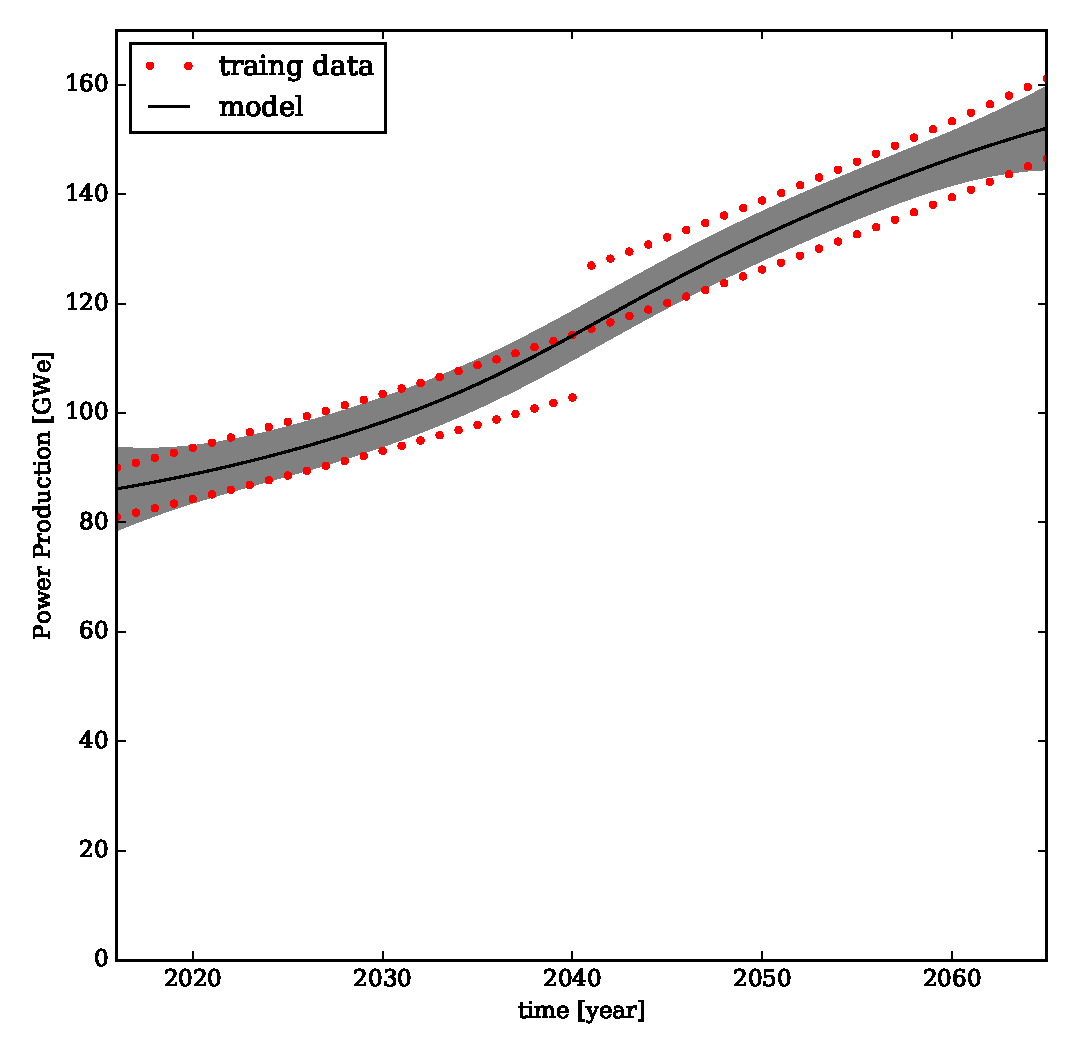
\includegraphics[width=0.9\textwidth]{gwe-model-.eps}
\caption{The Gaussian process model of a 1\% growth curve along with the
an initial 10\% under production followed by a 10\% under production. 
The model is represented by the black line that runs between the red 
training points. Two standard deviations form the model are displayed as the
gray region.}
\label{gwe-model-}
\end{figure}

The simple example above does not take advantage of an important 
feature of Gaussian processes. Namely, it is not limited to two production
curves in the training set.  As many as desirable may be used.  This will
allow the WORG algorithm to dynamically adjust the number of $Z$ simulations 
are used to predict the next deployment schedule. This allows WORG to 
effortlessly expand $Z$ when new, useful simulations yield valuable production
curves.  However, it also allows $Z$ to contract to discard production
curves that would drive the deployment schedule away from an optimum.

Now that the Gaussian process regression and dynamic time warping tools have 
been added to the toolbox, the architecture of the WORG algorithm can 
itself be examined.

\clearpage


\section{Selecting Deploytment Schedule Estimates}
\label{selecting}
\section{Performance \& Results}
\label{results}

To demonstrate the three variant WORG methods, an unconstrainted once 
through fuel cycle is modeled with the Cyclus simulator 
\cite{DBLP:journals/corr/HuffGCFMOSSW15}. In such a scenario, uranium
mining, enrichment, fuel fabrication, and storage all have effectively 
infinite capacities. The only meaningful constraints on the system are
how many light-water reactors (LWR) are built.

The base simulation begins with 100 reactors in 2016 that each produce
1 GWe, have an 18 month batch legnth with a one month reload time.
The initial fleet of LWRs retires evenly over the 40 years from 2016 to 
2056. All new reactors have a 60 year life time.  The simulation itself 
follows 50 years from 2016 to 2066. \emph{In situ} time horizons are 
expected to be much lower, on the order of 5, 10, or 20 years.

The study here compares how WORG performs from 0\% (steady state), 1\%, 
and 2\% growth curves from an initial 90 GWe target. These are examined
using the three estimation variants.  Calling $r$ the growth rate as a 
fraction, the demand curve is thus,
\begin{equation}
\label{f-rate}
f(t) = 90 (1 + r)^t
\end{equation}
Moreover, the upper bound for the number of deployable facilities at 
each time is set to be the ceiling of four times the total growth. 
That is, assuming four facilities at most could be deployed in the first
year, increase the upper bound along with the growth rate.  This yields
the following expression for $N$.
\begin{equation}
\label{n-rate}
N(t) = \left\lceil 4 (1 + r)^t\right\rceil
\end{equation}
The lower bound for the number of deployed reactor is simply set to the 
zero vector, $M = \mathbf{0}$.
%\section{Gaussian Process Regression}
\label{gp}

Evaluating the production curve for a specific kind of facility using 
full fuel cycle simulations is relatively expensive, even in the 
computationally cheapest case. This is because a fuel cycle realization 
typically computes many features that, though coupled to the production 
curve, are not directly the production. For example, the mass balance of 
fuel cycle physically bounds the electricity production. However, the 
mass balances are not explicitly taken into account when trying to meet
a demand curve.

Alternatively, surrogate models that predict the production curve directly
have many orders-of-magnitude fewer operations by virtue of not computing
implicit physical characteristics. This is not to say that the surrogate 
models are correct.  Rather, they are simply good enough to drive an 
optimization. Surrogate models are used here inform a simulator about where
in the parameter space to look next. Truth about production curves should
still be derived from the fuel cycle simulator and not the surrogate model.
In the WORG algorithm here, Gaussian processes are used to form the model. 

Gaussian processes are more fully covered elsewhere 
\cite{rasmussen2006gaussian}. Using Gaussian process for optimization has 
also been previously explored \citeme, though such studys tend not to 
investigate the intergal problems posed by facility deployment. As with 
dynamic time warping, a minimal but sufficient introduction to GP given for 
the purposes of the deployment optimization method here.
Conside the case of $Z$ simulations indexed by $z$ that each have a 
$\Theta_z$ deployment schedule and $g_z(t, \Theta_z)$ production curve.

A Gaussian process of these $Z$ simulations is set by its mean and 
covariance functions. The mean function is denoted as $\mu(t, \Theta)$ and 
is the expectation value $\E$ of 
the $G$ inputs:
\begin{equation}
\label{G}
G = \left\{g_1(t, \Theta_1), g_2(t, \Theta_2), \ldots, 
           g_Z(t, \Theta_Z)\right\}
\end{equation}
The covariance function is denoted $k(t, \Theta, t^\prime, \Theta^\prime)$ 
and is the expected value of the input to the mean. These can be expressed as
in Equations \ref{mean-func} \& \ref{covar-func}.
\begin{equation}
\label{mean-func}
\mu(t, \Theta) = \E G
\end{equation}
\begin{equation}
\label{covar-func}
k(t, \Theta, t^\prime, \Theta^\prime) = 
    \E\left[(g_z(t, \Theta) - \mu(t, \Theta))
            (g_z(t^\prime, \Theta^\prime) - \mu(t^\prime, \Theta^\prime))
      \right]
\end{equation}
Note that in the above, the Gaussian process is itself $P+1$ dimensional, 
since the means and covariance are a function of both the deployment 
schedule ($P$) and time ($+1$).

The Gaussian process $\GP$ approximates the production curve 
given $Z$ simulators. Allow $*$ to indicate that the a quantity comes from 
the model as opposed to coming from the simulator information. A model 
production curve can then be written using either functional or operator
notation, as appropriate:
\begin{equation}
\label{gp-def-approx}
g_*(t, \Theta) \approx \GP\left(\mu(t, \Theta), 
                                 k(t, \Theta, t^\prime, \Theta^\prime)\right) 
                \equiv \GP G
\end{equation}
In machine learning terminology, $G$ serves as the training set for the 
GP model.

Now, when performing a regression on Gaussian processes, 
the nominal functional form for the covariance must be given. 
Such a functional form is also known as the the kernel function.
The kernel contains the \emph{hyperparameters} that are solved for to 
obtained a best-fit Gaussian process. The hyperparameters themselves are
defined based on the definition of the kernel function. Hyperparameter 
values are found via a regression of the maximal likelihood of 
the production curve. Any functional form could potentially serve as a kernel
function. However, a generally useful form is the is the exponential 
squared. This kernel can be seen in Equation \ref{exp2-kernel} with 
hyperparameters $\ell$ and $\sigma^2$ for a vector of parameters $r$:
\begin{equation}
\label{exp2-kernel}
k(r, r^\prime) = \sigma^2 \exp\left[-\frac{1}{2\ell}(r - r^\prime)^2 \right]
\end{equation}
However, other kernels such as the Mat\'ern $3/2$ kernel and Mat\'ern $5/2$
kernel \cite{paciorek2004nonstationary} were observed to be more robust for 
the WORG method. These can be seen in Equations \ref{matern-32} and 
\ref{matern-52} respectively.
\begin{equation}
\label{matern-32}
k(r, r^\prime) = \sigma^2 
                 \left(1 + \frac{\sqrt{3}}{\ell}|r - r^\prime|\right)
                 \exp\left(-\frac{\sqrt{3}}{\ell}|r - r^\prime|\right)
\end{equation}
\begin{equation}
\label{matern-52}
k(r, r^\prime) = \sigma^2 
                 \left(1 + \frac{\sqrt{5}}{\ell}|r - r^\prime|
                         + \frac{5}{3\ell^2}|r - r^\prime|^2\right)
                 \exp\left(-\frac{\sqrt{5}}{\ell}|r - r^\prime|\right)
\end{equation}

From here, say that $\K$ is a covariance matrix $\K$ 
such that the element at the $r$-th row and $r^\prime$-th column is 
given by a choice of kernels seen in 
Equations \ref{exp2-kernel}-\ref{matern-52}. Then the 
log likelihood $\log q$ of the obtaining the training set production curves 
$G$ for a given time grid $\mathbf{t}$ and deployment schedule is as follows.
\begin{equation}
\label{log-q}
\log q(G|\mathbf{t}, \Theta) 
    = -\frac{1}{2}G^\top\left(\K + \tau^2\I\right)^{-1}G
      -\frac{1}{2}\log\left|\K + \tau^2\I\right|
      -\frac{ZTP}{2}\log 2\pi
\end{equation}
Here, $\tau$ is the uncertainty in the production curves coming from the 
simulations themselves. As most simulators do not report such uncertainties, 
$\tau$ may be set to floating point precision. $\I$ is the usual identity 
matrix. The hyperparameters $\ell$ and $\sigma^2$ are then adjusted via 
standard optimization methods such that Equation \ref{log-q} is minimized. 
This regression of the Gaussian process itself yields the most likely 
model of the production curve, knowing only a limited number simulations.

However, the purpose of such a Gaussian process regression is to evaluate 
the production curve at points in time and for deployment schedules that 
have not been simulated. Take a time grid $\mathbf{t_*}$ and a hypothetical
deployment schedule $\Theta_*$. Now call the covariance vector between
the training set and the model evaluation    
$\mathbf{k}_* = \mathbf{k}(\mathbf{t_*}, \Theta_*)$. 
The production curve predicted by this Gaussian process is then given by
the following:
\begin{equation}
\label{metric-model}
\mathbf{g}_*(\mathbf{t}_*, \Theta_*) = 
    \mathbf{k}_*^\top \left(\K + \tau^2\I\right)^{-1}G
\end{equation}
Equations \ref{mean-func}-\ref{metric-model} are derived in detail and
generality in \cite{rasmussen2006gaussian}. 

However, implementing the above for the specific case of the WORG algorithm 
is not needed.  Off-the-shelf Gaussian process modeling software 
libraries already exist and are applicable to the regression problem here.
Scikit-learn v0.17 \cite{scikit-learn} and George v0.2.1 \cite{hodlr} 
implement such a method and have a Python interface. George is specialized 
around Gaussian processes, and thus is preferred for WORG over scikit-learn, 
which is a general purpose machine learning library.

As an example, consider a Gaussian process between two power production 
curves. The first is a nominal 1\% growth in GWe for 50 years starting at 
90 GWe in 2016. The second curve under produces the first curve by 10\% 
for the first 25 years and over produces by 10\% for the last 25 years.
Additionally, assume that there is a 10\% error on the training data set.
This will produce a model of the mean and covariance that splits the 
difference between these two curves. This example may be seen graphically
in Figure \ref{gwe-model-}.

\begin{figure}[htb]
\centering
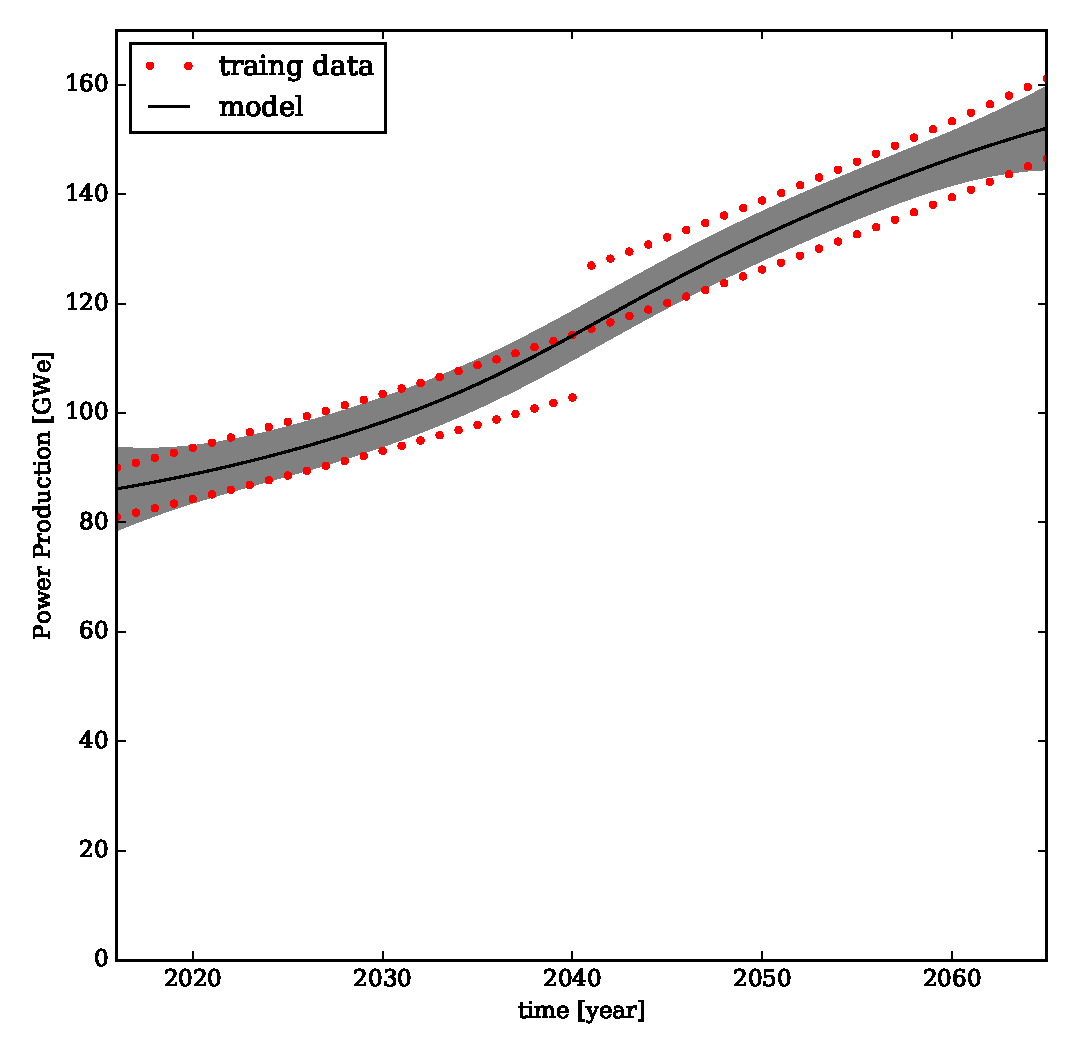
\includegraphics[width=0.9\textwidth]{gwe-model-.eps}
\caption{The Gaussian process model of a 1\% growth curve along with the
an initial 10\% under production followed by a 10\% under production. 
The model is represented by the black line that runs between the red 
training points. Two standard deviations form the model are displayed as the
gray region.}
\label{gwe-model-}
\end{figure}

The simple example above does not take advantage of an important 
feature of Gaussian processes. Namely, it is not limited to two production
curves in the training set.  As many as desirable may be used.  This will
allow the WORG algorithm to dynamically adjust the number of $Z$ simulations 
are used to predict the next deployment schedule. This allows WORG to 
effortlessly expand $Z$ when new, useful simulations yield valuable production
curves.  However, it also allows $Z$ to contract to discard production
curves that would drive the deployment schedule away from an optimum.

Now that the Gaussian process regression and dynamic time warping tools have 
been added to the toolbox, the architecture of the WORG algorithm can 
itself be examined.

\clearpage

%\subsection{Dynamic Time Warping}
\label{dtw}

The question of how to take the difference between the demand curve and 
the production curve is an important one. The na\"ive option is to simply 
take the $L_1$ norm of the difference between these two time sereies, as 
seen in Equation \ref{delta-l1}.  However, since $g(t, \Theta)$ for 
a simulation is expensive compute, any operation that can meaningfully 
exacerbate the difference betweeen time series helps drive down the number 
of optimization iterations.

Dynamic time warping is just such a mechanism. It computes 
a distance between any two time series which compounds the separartion 
between the two. Additionally, the time series are not required to be of the 
same length, though for optimization purposes there is no reason for them 
not to be. DTW gives a measure of amount that one time series would need to 
be warped to become the other time series. It is, therefore, a holistic  
measure that operates over the complete time series. Dynamic time warping
is more fully covered in \cite{muller}.  However, an 
optimization-relevant introduction is given here.

For the time series $f$ and $g$, there are three parts to dynamic time 
warping. The first is the distance $d$, which will be minimized. The second 
is a cost matrix $C$ that helps compute $d$ by indicating how far a point 
on $f$ is from another point on $g$. Thirdly, the warp path $u$ is the 
minimal cost curve through the $C$ matrix from the fist point in time to 
the last. The DTW distance can thus be interpreted as the 
total cost of travelling the warp path.

The first step in computing a dynamic time warp distance is to 
assemble the cost matrix. Say that the demand time series $f$ has 
length $A$ indexed by $a$ and the production time series $g$ has 
length $B$ indexed by $b$. For the optimization problem here, $A$ and $B$
are in practice both equal to $T$.  However, it is useful to have $a$ and 
$b$ index the two time series separately. Now denote an $A\times B$ matrix 
$\Delta L$ as the $L_1$ norm of the difference between $f$ and $g$:
\begin{equation}
\label{delta-l1}
\Delta L_{a,b} = \left|f(a) - g(b, \Theta)\right|_1
\end{equation}
The cost matrix $C$ may now be defined as the $A\times B$ sized matrix 
which follows the recursion relations seen in Equation \ref{cost-matrix}.
\begin{equation}
\label{cost-matrix}
\begin{split}
C_{1,1} & = \Delta L_{1,1}\\
C_{1,b+1} & = \Delta L_{1,b} + C_{1,b}\\
C_{a+1,1} & = \Delta L_{a,1} + C_{a,1}\\
C_{a+1,b+1} & = \Delta L_{a,b} + \min\left[C_{a,b}, C_{a+1,b}, C_{a,b+1}\right]
\end{split}
\end{equation}
The boundary conditions above are the same as setting an infinite cost to 
any $a \le 0$ or $b \le 0$. The cost matrix $C$ has the same units as the 
demand curve. However, the scale of $C$ is (except for the fiducial case) 
larger than the demand. This is because the cost matrix compounds the 
minimum value of previous entries. 

Knowing a cost matrix, the warp path can be computed by traversing the 
matrix backwards from the $(A, B)$ corner to the $(1, 1)$ corner.
If the length of the warp is $I$ indexed by $i$, the warp path itself 
can be thought of as a sequence of coordinate points $u_i$. For a given 
point $u_i$ in the warp path, the previous point $u_{i-1}$ found by 
picking the minimum cost point among the locations one column over $(a,b-1)$, 
one row over $(a-1,b)$, and one previous diagonal element to $(a-1,b-1)$. 
Equation \ref{warp-path} expresses this mathematically.
\begin{equation}
\label{warp-path}
u_{i-1} = \argmin\left[C_{a-1,b-1}, C_{a-1,b}, C_{a,b-1}\right]
\end{equation}
The maximum possible length of $u$ is thus $\max(I) = A + B$.
The minimum possible length, though, is $\min(I) = \sqrt{A^2 + B^2}$. 

The dynamic time warping distance distance $d$ can now be stated as the 
cost of the final entry of the warp path normalized by the maximum possible
length of the warp path.  
\begin{equation}
\label{d-calc-ab}
d(f, g) = \frac{C_{A,B}}{A + B}
\end{equation}
However, because the demand curve and the production curve that is predicted
or calculated are typically defined on the same time grid, $d$ can be further
reduced to the following:
\begin{equation}
\label{d-calc}
d(f, g) = \frac{C_{T,T}}{2T}
\end{equation}
Therefore, $d$ has the same units as the demand curve, production curve, 
and cost matrix.

As an example, take 1\% growth that starts with 90 GWe in the year 
2016 as the demand curve. Then consider a production curve that 
under produces the demand by 5\% for 25 years before switching to over 
producing this curve by 5\% for the next 25 years.  
Figure \ref{cost-demand-to-production} shows the dynamic time warping 
between these two.

\begin{figure}[htb]
\centering
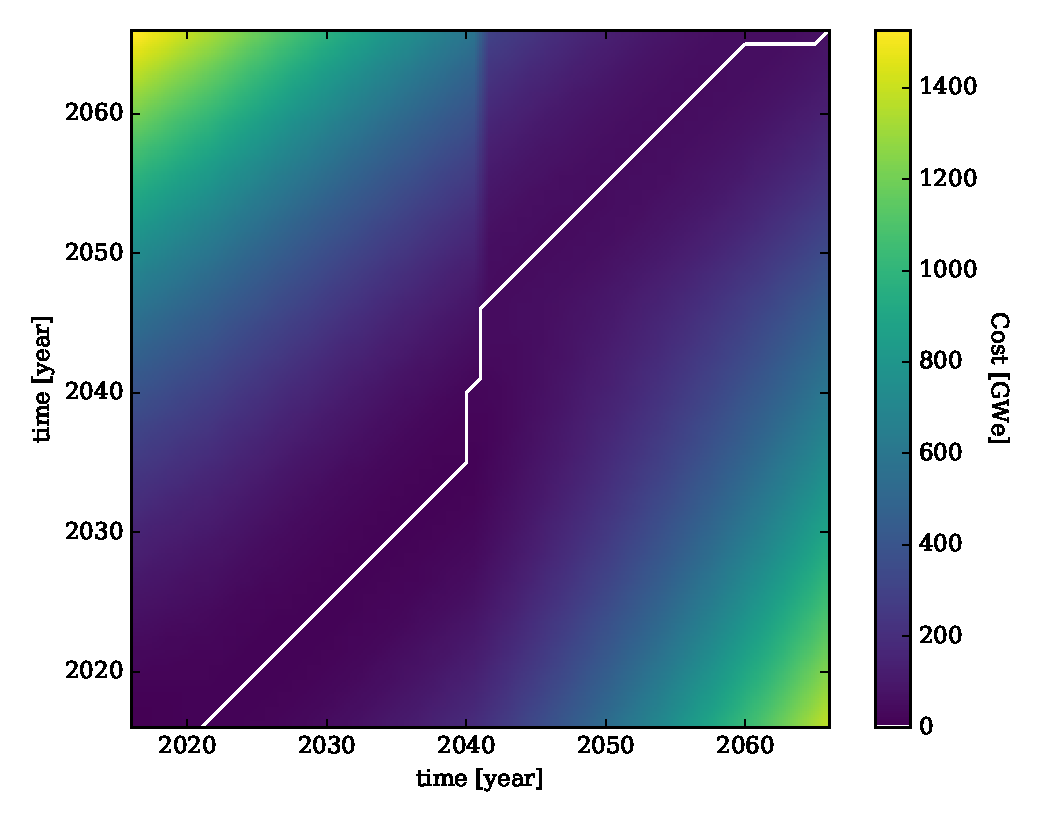
\includegraphics[width=0.9\textwidth]{cost-demand-to-production.eps}
\caption{Heat map of the cost matrix between a 1\% growth demand curve and 
a production curve the under produces by 5\% for the first 25 years and then
over produces for the second 25 years.  
The warp path $u$ is superimposed as the white curve on top of the 
cost matrix.}
\label{cost-demand-to-production}
\end{figure}

Additionally, the warp path between the example demand and production 
curves is presented as the white curve on top of the heat map in 
Figure \ref{cost-demand-to-production}. 
Recognize that $u$ is monotonic along both time axes. Furthermore, the precise
path of $u$ minimizes the cost matrix at every step. Regions of increased 
cost in the cost matrix have the repel the warp path. Incidentally, the 
distance $d$ between the demand and production curves happens 
to be 0.756 GWe.

Dynamic time warping distance can therefore be used as an objective function 
to minimize for any demand and production curves. However, using full 
simulations to find $g(t, \Theta)$ remains expensive, even though DTW itself 
is computationally cheap. Therefore, a mechanism to reduce the overhead 
from production curve evaluation is needed.

\section{Conclusions \& Future Work}
\label{conclusion}

%% Uncomment the following to use.
\section*{Acknowledgements}
\label{acknow}


%%%%%%%%%%%%%%%%%%%%%%%%%%%%%%%%%%%%%%%%%%%%%%%%%%%%%%%%%%%%%%%%%%%%%%%%%%%%%%%%
\bibliographystyle{ans}
\bibliography{refs}
\end{document}
